\section{Podział projektu}
{Wykorzystanie wielu języków programowania (Java, C\#, Python, JavaScript, Android, TypeScript) wymagało podziału projektu ze względu na użyte technologie oraz ich zastosowania w aplikacji. Miało to między innymi duży wpływ na szybszą fazę wytwarzania oprogramowania, jak i łatwość zrozumienia kodu. Wykorzystanie innej koncepcji mogłoby spowodować bardzo wolne działanie środowiska programistycznego lub problemy z późniejszą naprawą błędów. Każda z aplikacji poprzez strukturę katalogową lub podprojektową wydzielała logiczne części podprojektu. Tabela \ref{architecture} przedstawia szczegółowy podział użytych technologii niezbędnych do stworzenia systemu.
	
		\begin{table}[htbp]
		\caption{Podział technologii}
		\label{architecture}
		\begin{center}
			\begin{tabular}{ | p{4cm}| p{3cm} | p{6cm} |}
				\hline Nazwa podprojektu & Technologia &  Zastosowanie \\ \hline   
				\hline  Aplikacja mobilna &  Ionic - TypeScript & Aplikacja mobilna służąca do tworzenia oraz przesyłania zdjęć półek sklepowych oraz prezentacji danych wynikowych.\\ \hline
				
				\hline  Mikroserwis przetwarzania obrazu & Python & Mikroserwis służący do klasyfikacji obiektów występujących na obrazie oraz informacji o nich - pozycji, nazwie.\\ \hline
				
				\hline Mikroserwis zasad obiektów klasyfikacji \mbox{bazodanowy} & Java & Mikroserwis służący do przetwarzania wyników otrzymanych z~mikroserwisu analizy obrazu przy użyciu sieci semantycznej.\\ \hline
				
				\hline Aplikacja internetowa & ASP.NET Core & Aplikacja internetowa odpowiedzialna za przetwarzanie żądań kierowanych z aplikacji mobilnych oraz zarządzanie przepływem danych pomiędzy mikroserwisami.\\ \hline
			\end{tabular}
		\end{center}
	\end{table}	
	
	
Projekt zarządzający komunikacją pomiędzy aplikacją mobilną a mikroserwisami wymagał dodatkowego użycia podmodułów. Warstwy aplikacji w~tym przypadku tworzyły logiczną całość aplikacji internetowej oraz ułatwiały wprowadzanie nowych zmian lub zrozumienie kodu przez innych. Tabela \ref{project-architecture} przedstawia opis poszczególnych modułów systemu.


\begin{table}[htbp]
	\caption{Opis poszczególnych modułów aplikacji}
	\label{project-architecture}
	\begin{center}
		\begin{tabular}{ | p{3cm}| p{3cm} | p{6cm} |}
			\hline Nazwa modułu & Typ &  Opis \\ \hline   
			
			\hline  Moduł aplikacji internetowej REST &  Aplikacja ASP.NET Core MVC & Moduł odpowiedzialny za przechwytywanie oraz przetwarzanie żądań HTTP kierowanych z aplikacji mobilnej. Jest to moduł uruchamiający pozostałe podmoduły oraz zawierający ich konfigurację.\\ \hline
			
			\hline  Moduł logiki biznesowej & Biblioteka klas & Moduł zawierający klasy odpowiedzialne za przetwarzanie danych odbieranych w punktach dostępowych aplikacji internetowych. \\ \hline
			
			\hline Moduł struktur bazodanowych \mbox{bazodanowy} & Biblioteka klas & Moduł zawierający deklarację tabel bazodanowych oraz konfigurację bazy danych.\\ \hline
			
			\hline Moduł komunikacji & Biblioteka klas & Moduł zawierający konfigurację połączeń z pozostałymi mikroserwisami oraz modele komunikacji pomiędzy nimi.\\ \hline
			
			\hline Moduł modeli & Biblioteka klas & Moduł zawierający przetwarzane modele aplikacji.\\ \hline
			
			
			\hline Moduł konwersji danych & Biblioteka klas & Moduł zawierający logikę umożliwiającą konwersję modeli przetwarzanych przez aplikację na modele bazodanowe lub komunikacyjne wykorzystywane przez Mikroserwisy\\ \hline

		\end{tabular}
	\end{center}
\end{table}	

W związku z podziałem projektu na podprojekty oraz podmoduły można wyróżnić rozbudowaną architekturę systemu oraz widoczny zakres obowiązków poszczególnych podprojektów. Szczegółowy opis ich architektury wraz z~wykorzystaną technologią został zamieszczony w kolejnych podrozdziałach.}


\section{Komunikacja}
{Wykorzystanie wielu technologii oraz języków programowania uniemożliwiało użycie wzorca projektowego zwanego monolitem. Zakłada on między innymi przepływ danych w obrębie jednej aplikacji, co w tym przypadku spowodowałoby duże problemy z obsługą błędów, przetwarzaniem wyników bibliotek oraz zwiększyłoby znacząco czas wytwarzania oprogramowania. W związku z~tym zdecydowano się na zastosowanie architektury mikroserwisów, w których każda z aplikacji stanowi osobny niezależny byt w hierarchii. W przypadku gdy jedna z aplikacji zostanie wyłączona lub napotka na nieoczekiwany błąd uniemożliwiający jej pracę, całość projektu może dalej przetwarzać dane, a~użytkownik końcowy może nie dostrzec błędów. Wykorzystanie architektury mikroserwisów wymusza komunikację aplikacji przy pomocy wybranego protokołu komunikacyjnego, którym może być HTTP lub AMQP(Advanced Message Queuing Protocol)\cite{AMQP}. Jednym z priorytetów stawianych podczas projektowania aplikacji była szybkość przetwarzania danych. W związku z tym uznano, że protokół AMQP, który jest przystosowany do rozwiązań Internetu Rzeczy, umożliwi znacznie szybszą komunikację niż konieczność przetwarzania żądań HTTP. 
	
	
Rozwiązanie oparte o architekturę rozproszoną mikroserwisów pozwala nie tylko na wykorzystanie dowolnego języka programowania lub środowiska uruchomieniowego. Dzięki niemu możliwe jest zwiększenie mocy obliczeniowej dostępnej podczas przetwarzania danych w aplikacji poprzez wykorzystanie więcej niż jednej maszyny. W przypadku braku odpowiedniej ilości zasobów na jednym z komputerów architektura zakłada możliwość podpięcia kolejnych agentów, które mogą przetwarzać dane oraz dostarczyć rezultat. W tym przypadku, każdy z nich musi połączyć się do jednego centralnego węzła komunikacyjnego tworzonego przez RabbitMQ \cite{RabbitMQ} - systemu kolejkowego.

Każdy z mikroserwisów korzysta z jednej zdefiniowanej kolejki, do której przesyłane są wiadomości wraz z danymi - product-scanner-api. Aby wiadomość trafiła do odpowiedniego mikroserwisu, wykorzystywany jest tak zwany routing-key, czyli wskazanie agentów, które nasłuchują w określonym celu. System oparty jest o konieczność potwierdzenia odebrania oraz przetworzenia danych przez pozostałe mikroserwisy. W przypadku napotkania awarii system spróbuje co najmniej dwa razy ponownie wysłać wiadomość. Dane przesyłane pomiędzy serwisami są przekazywane w postaci bajtów, w których znajduje się plik formatu JSON \cite{JSON}. 
}
	
	
\section{Aplikacja internetowa - Gateway}	
{	Rozbicie architektury aplikacji internetowej na kilka podmodułów wymagało zastosowania odpowiednich wzorców projektowych oraz przemyślanej struktury aplikacji. Jednym ze wzorców projektowych, który świetnie sprawdza się w tego typu aplikacjach, jest wzorzec "odwróconego sterowania", znany pod nazwą "dependency injection". Jego wykorzystanie pozwoliło między innymi na przekazywanie do konstruktorów klas stworzonych wcześniej instancji obiektów. Dzięki temu obiekt połączenia do bazy danych tworzony był tylko raz podczas przetwarzania zapytania i mógł być używany w pozostałych podprojektach. Zastosowanie wzorca architektonicznego umożliwiło zmniejszenie rendundancji kodu, która powstała na skutek konieczności ciągłej inicjalizacji obiektów. Ponadto dobrą praktyką, do której powinien stosować się każdy programista, jest możliwość reużywalności kodu, na co z pewnością pozwala zastosowany wzorzec. 

Aplikacja mobilna w celu komunikacji używa protokołu HTTP. W związku z tym 	 przygotowano moduł umożliwiający przetwarzanie kierowanych żądań HTTP zgodnie ze wzorcem architektonicznym REST (Representational State Transfer). Aplikacja internetowa zawiera bezstanowe kontrolery, które konwertują dane wysłane z telefonu w postaci JSON oraz przekazują je do dalszego przetwarzania przez aplikację. Wzorzec architektoniczny zakłada między innymi sposób tworzenia adresów URL według dostępów do zasobów oraz zgodnie z metodą HTTP. Żądanie kierowane pod odpowiedni zasób powoduje przekazanie zależności odpowiedniego punktu docelowego do konstruktora kontrolera przetwarzającego dane oraz przekazanie informacji do serwisu odpowiedzialnego za zasób. Odpowiedź kontrolera jest zależna od typu przesłanego zapytania. W przypadku utworzenia zasobów może być nią status kod 201 oznaczający pomyślnie stworzony zasób w systemie. Ze względu na bardzo istotną rolę jaką pełnią kontrolery w aplikacjach internetowych, ilość kodu znajdującego się w nich powinna być zmniejszona do minimum. Ich przeznaczeniem jest przyjęcie żądania oraz przekazanie do dalszego przetwarzania, stąd nacisk na przeniesienie logiki biznesowej aplikacji do osobnego modułu.

Dalsze przetwarzanie danych aplikacji odbywa się w serwisach, czyli klasach odpowiedzialnych za przetwarzanie logiki biznesowej. Do ich odpowiedzialności należy między innymi zapis danych w bazie danych lub przesłanie ich do mikroserwisów. Serwisy, tak samo jak i kontrolery, wykorzystują wzorzec odwróconego sterowania, aby otrzymać niezbędne zależności konieczne do poprawnego przetworzenia danych. W celu zmniejszenia redundancji kodu wykorzystano typy generyczne oraz stworzono bazowe implementacje serwisów. Zawiera ona kod, powtarzalny dla każdego serwisu - między innymi konwersję plików lub zapis danych w tabeli bazodanowej. 

Logika serwisu może zawierać wywołanie mikroserwisu w innej technologii. W tym przypadku pomyślne zapisanie w bazie danych może powodować zgłoszenie do mikroserwisu gotowości do przetwarzania obrazu lub informacji. W tym celu mechanizm odwróconego sterowania przekazuje obiekt komunikacji AMPQ do konstruktora serwisu. Nazwa przekazanego obiektu do metody publikacji wiadomości przy użyciu mechanizmu refleksji umożliwia wskazanie pasma komunikacyjnego (routing-key), na który zostanie wysłana wiadomość. W przypadku otrzymania wiadomości zwrotnej moduł zarządzania komunikacją mikroserwisów posiada klasy odpowiadające za przechwytywanie zdarzeń przesłanych do aplikacji. 

Komunikacja z aplikacją internetową przy pomocy architektury REST nie umożliwia wymiany danych w czasie rzeczywistym. Dodatkowo wykorzystanie mikroserwisów zezwala na rozbicie aplikacji na wiele niezależnych podaplikacji, jednak nie pozwala na predykcję czasu przetworzenia danych. Tworząc zasób, użytkownik w najgorszym przypadku nie otrzyma wszystkich danych, na których mu zależy w trakcie pierwszego dostępu do widoku. W związku z tym zastosowano komunikację przy użyciu gniazdek www oraz technologię SignalR \cite{SignalR}. Przechwycone zdarzenie pozwala na rozpowszechnienie danych do wszystkich klientów podłączonych do aplikacji. Połączenie to wymaga, aby klient - aplikacja mobilna, łączył się do systemu wraz z początkiem korzystania z aplikacji. Wykorzystanie technologii gniazdek pozwala na dodatkowe rozproszenie komunikacji oraz obsługę żądań wielu użytkowników w tym samym czasie.

\section{Aplikacja mobilna}
{ Użytkownicy systemu dostarczają zdjęcia poddawane przetwarzaniu oraz wnioskowaniu przy użyciu aplikacji mobilnej. Tworząc rozwiązanie działające na telefonach komórkowych należy uwzględnić różne platformy oraz architektury docelowych urządzeń. Ze względu na wykorzystanie aplikacji do prezentacji danych oraz przesyłanie zdjęć z galerii skorzystano z rozwiązania hybrydowego kosztem aplikacji natywnej. Wiąże się to z brakiem dostępu do bibliotek, które współpracują bezpośrednio z podzespołami urządzenia, ale przyspiesza w znaczący sposób wytwarzanie oprogramowania na wiele platform. Aplikacja może działać na systemach operacyjnych iOS oraz Android. Stworzono ją przy użyciu bibliotek Ionic \cite{Ionic}, które bazują na modelu Cordova \cite{Cordova}. W celu prezentacji danych skorzystano z biblioteki Angular\cite{Angular} w wersji 5. Aplikacja może również działać na innych platformach (na przykład przeglądarce), jednakże jej najważniejsza funkcjonalność, czyli możliwość przetwarzania zdjęć, będzie wtedy niedostępna.
	
Aplikacja mobilna generuje widoki w oparciu o dane dostępne na serwerze. Komunikacja z aplikacją internetową odbywa się przy użyciu protokołu HTTP. Urządzenia mobilne podłączone do sieci, posiadają swoją własną kartę sieciową oraz adres IP różny od używanego przez serwer. Spowodowało to konieczność odblokowania połączeń do serwera z innych domen niż ta używana przez aplikację internetową. W związku z tym na serwerze www uruchomiono obsługę CORS \cite{CORS} (Cross-Origin Resource Sharing) co pozwoliło na komunikację HTTP z innych urządzeń niż maszyna aplikacji. 

Tworzenie aplikacji mobilnej przy użyciu biblioteki Angular wymusza na programiście znajomość oraz stosowanie wzorców projektowych takich jak reaktywne programowanie. Dzięki temu zmiana wartości zmiennych klas przypisanych do komponentów w drzewie DOM spowoduje zmianę danych wyświetlanych użytkownikowi. Proces wiązania danych poprzez zastosowanie typów obserwowanych może być uciążliwy dla programistów przyzwyczajonych do operacji asynchronicznych używanych na platformach uruchomieniowych .NET lub NodeJS. Jednakże jego opanowanie w pełni wykorzystuje możliwości, które niesie ze sobą wykorzystanie asynchronicznych operacji.
}
\section{Mikroserwis przetwarzania obrazu}
{ Aplikacje używające algorytmów uczenia maszynowego korzystają z wcześniej stworzonych modeli, w których zawarte są dane oraz reguły wykorzystywane przez bibliotekę Tensorflow. W przypadku mikroserwisu do przetwarzania obrazu model zawiera informacje dotyczące klasyfikacji przedmiotów znajdujących się na obrazach. Zdjęcia, które posłużyły jako wejście aplikacji, zostały umieszczone na repozytorium w katalogu mikroserwisu do przetwarzania obrazu w folderze images. Ze względu na charakterystykę sposobu działania aplikacji pod względem przetwarzania obrazu, model użyty do klasyfikacji musi zostać wczytany do pamięci oraz wykorzystywany przy każdym wywołaniu mikroserwisu. Zostało to wymuszone między innymi poprzez wywoływanie metod przetwarzania obrazu w zdarzeniach otrzymywanych przez klienta kolejki RabbitMQ. Otrzymanie wiadomości wraz z danymi do interpretacji umożliwia wywołanie metod wnioskujących i klasyfikujących. Efektem uzyskanych operacji jest zdjęcie wynikowe z wykrytymi przedmiotami i ich opisem oraz dane dotyczące ich położenia. Zakończenie działania mikroserwisu skutkuje przygotowaniem wiadomości wysyłanej do aplikacji internetowej wraz z informacją o~znalezionych przedmiotach, ich położeniu względem osi X i Y oraz ocenie dokonanej klasyfikacji. Dane te mogą posłużyć do przeprowadzenia wnioskowania przy użyciu ontologii zdefiniowanej w mikroserwisie reguł semantycznych.
\newpage
W celu demonstracji przykładu działania mikroserwisu zostaną zaprezentowane zdjecia pokazujące sposób działania algorytmu. Poniższe obrazy przedstawiają produkty w różnych warunkach użytkowania. Zdjęcia zostały stworzone z uwzględnieniem niekorzystnych warunków panujących w sklepach. Przykładowe dane wejściowe dla algorytmu zostały przedstaione na obrazach z Rysunku \ref{beforeClasification}.

\begin{figure}[htb]
	\caption{Próbki obrazów poddane klasyfikacji produktów.}
	\label{beforeClasification}
	\noindent\begin{minipage}
		{0.43\textwidth}\raggedleft		\includegraphics[width=\linewidth]{"images/detection_sample"}
	\end{minipage}
	\begin{minipage}{0.57\textwidth}
		\includegraphics[width=\linewidth]{"images/detection_sample2"}
	\end{minipage}
\end{figure}

Mikroserwis dzięki zastosowaniu bibliotek analizy obrazu umożliwi na detekcje przedmiotu oraz jego klasyfikacje. Wynik algorytmu został przedstawiony na Rysunku \ref{afterClasification}. Prostokąt, znajdujący się na obrazie otacza wykryty przedmiot. Algorytm umożliwia dodanie do obrazu wyniku klasyfikacji w postaci jego nazwy. Ponadto wynik przetwarzania zawiera informacje o położeniu prostokątów w postaci tablicy danych.


\begin{figure}[htb]
	\caption{Wynik klasyfikacji produktów.}
	\label{afterClasification}
	\noindent\begin{minipage}
		{0.43\textwidth}\raggedleft		\includegraphics[width=\linewidth]{"images/detection_sample_result"}
	\end{minipage}
	\begin{minipage}{0.57\textwidth}
		\includegraphics[width=\linewidth]{"images/detection_sample_result2"}
	\end{minipage}
\end{figure}
}
\section{Mikroserwis reguł semantycznych}
{
W celu wnioskowania oraz dopasowywania odpowiednich reguł, które muszą spełnić przedmioty na obrazie, wykorzystano ontologię stworzoną w Protege \cite{Protege}. W bazie wiedzy zostały zawarte informacje dotyczące klasyfikowanych przedmiotów, ich cech oraz sprawdzanych reguł na obrazie. Dane zostały zapisane w trójkach RDF w formacie XML. Aplikacja zakłada istnienie ontologii wraz z regułami dotyczącymi przedmiotów, stworzonymi w przy użyciu języka SWRL\cite{SWRL} (Semantic Web Rule Language) w folderze aplikacji. Semantyka świata otwartego powoduje, że znalezienie przedmiotu na obrazie nie znajdującego się w bazie wiedzy powoduje brak wyników otrzymanych z wnioskowania.

Wnioskowanie przeprowadzone na istniejącym zbiorze danych wywoływane jest po wywołaniu zdarzenia wraz z danymi otrzymanymi z mikroserwisu przetworzenia obrazu. Elementem wywołującym zdarzenie jest aplikacja internetowa. Klasyfikatory otrzymane z analizy obrazu dodawane są do istniejącej ontologii, a następnie przeprowadzane jest na nich wnioskowanie. Umożliwi to automatyczne dopasowanie zbioru reguł oraz detekcje czy wszystkie istniejące reguły zostały spełnione na obrazie. Wynikiem działania mikroserwisu jest zbiór informacji o regułach, w których wystąpiła anomalia. Brak odpowiedzi serwisu, który mógłby być spowodowany chwilową niedostępnością serwera, nie powoduje braku możliwości wyświetlenia rezultatu przetwarzania użytkownikowi. Na ekranie telefonu komórkowego wówczas zostanie pokazana informacja o wykrytych przedmiotach. 

Ontologia przygotowana w programie Protege zawiera podstawowe elementy badane w przykładowej aplikacji. Została ona przedstawiona na rysunku \ref{ontology}. Do stworzonego modelu powstało wiele reguł przy użyciu języka SWRL.Dodatkowo, zapytania zostały wzbogacone o właściwości danych (Data properties) oraz o istniejące indywiduła. Bardzo dobrym przykładem jest wskazanie pozycji przedmiotu na obrazie. Reguła poza badaniem pozycji przy użyciu stałych dopasowyje obiekt istniejącej klasy Position - przykładowo "BottomPosition", oznaczająca dolne regiony obrazu. Mikroserwis podczas przetwarzania otrzymanych danych wykorzystuje interfejs programistyczny biblioteki JENA. Dzięki niemu dodawane są indywidua oraz przetwarzana jest istniejące ontologia wraz z nowym zbiorem informacji. Wynik zostaje przekształcony do postaci słownika zawierającego identyfikator obrazka oraz poszczególne cechy przedmiotu. Przetwarzanie ontologii ze względu na zapytania SWRL jest wykonywane przy użyciu mechanizmu "Pellet".

\begin{figure}[htb]
	\centering
	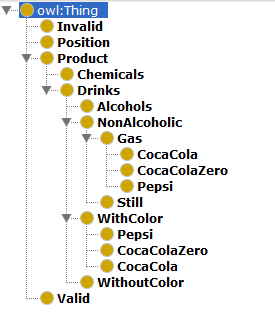
\includegraphics[width=0.5\linewidth]{../../../../Downloads/ontology}
	\caption[Ontologia]{Ontologia mikroserwisu reguł semantycznych.}
	\label{ontology}
\end{figure}

}
